\chapter{\label{chapter:FactoryManager}The Factory Manager}

The Factory Manager uses Factory classes to create objects for GMAT's model.  It takes creation
messages from the Moderator, passes those messages into the Factory designed to create the specific
type of object requested, and returns the created object to the Moderator.

This chapter describes the Factory Manager and introduces the Factory classes.  The Factory Manager
acts as the central junction into the Factory subsystem, managing Factories as they are created an
d registered, and routint creation requests to the specific Factory that knows how to create
a requested type of object.

Object creation is performed in a Factory derived from the Factory base class. An overview of the
Factory infrastructure is provided in Section~\ref{section:FactoryClasses}. Details about how you
use the Factory classes to extend GMAT can be found in Chapter~\ref{chapter:ExtendingGMAT}.

\section{Design Principles}

\subsection{Factory Manager Responsibilities}

\begin{enumerate}
\item Manages object creation for the engine.
\item Calls Factory classes to create objects.
\item Registers new Factories to support newly defined objects.
\item Provides a list of creatable object types.
\end{enumerate}

\subsection{The Abstract Factory Pattern, Factory Subclasses, and the Factory Manager}

\section{Design}

\begin{figure}[htb]
\begin{center}
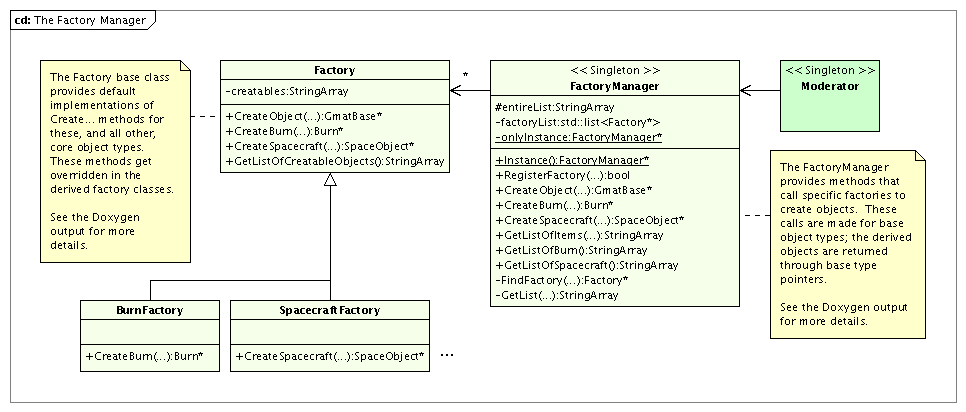
\includegraphics[460,197]{Images/TheFactoryManager.png}
\caption{The Factory Manager and Some Factories}
\label{figure:FactManClassDiagram}
\end{center}
\end{figure}



\subsection{Class Details}

\subsubsection{Class Attributes}

\subsection{\label{section:FactoryClassDesign}Design of the Factory Classes}

\subsubsection{Factory Details}


\section{Usage and Modification}

